A closed loop system has the characteristic equation given by \begin{align} s^3+Ks^2+(K+2)s+3 = 0 \end{align}For this system to be stable, which one of the following conditions should be satisfied? \\
(A) 0 \(<\) K \(<\) 0.5 
(B) 0.5 \(<\) K \(<\) 1 
(C) 0 \(<\) K \(<\) 1 
(D) K \(>\) 1 \\

\solution
Computing the Routh array for the given characteristic equation, we get-

\begin{align}
    \mydet{s^3 \\ s^2 \\ s \\ s^0} 
    \mydet{1 & K+2 & 0 \\ K & 3 & 0 \\ \frac{K^2+2K-3}{K} & 0 & 0 \\ 3 & 0 & 0}
\end{align}

According to the Routh-Hurwitz stability criterion, for the system to be stable there should be no sign changes in the first column of the Routh array. That means-
\begin{align}
    K > 0 \ \texttt{and} \ \frac{K^2+2K-3}{K} > 0 
\end{align}
\begin{align}
\Rightarrow K > 0 \ \texttt{and} \ (K-1)(K+3) > 0 
\end{align}
which gives us 
\begin{align}
    K > 0 \ \texttt{and} \ (K > 1 \ \texttt{or} \ K < -3).
\end{align}
Note that K cannot be negative.

\begin{align}
\Rightarrow K > 1 
\end{align}

The program to compute the routh-array and stabilty for different values of K.
\begin{lstlisting}
    codes/ee18btech11039/routh_array.py
\end{lstlisting}

The program for plotting the poles of the system for different values of K.
\begin{lstlisting}
    codes/ee18btech11039/pole_plot.py
\end{lstlisting}

\begin{figure}[!ht]
\begin{center}
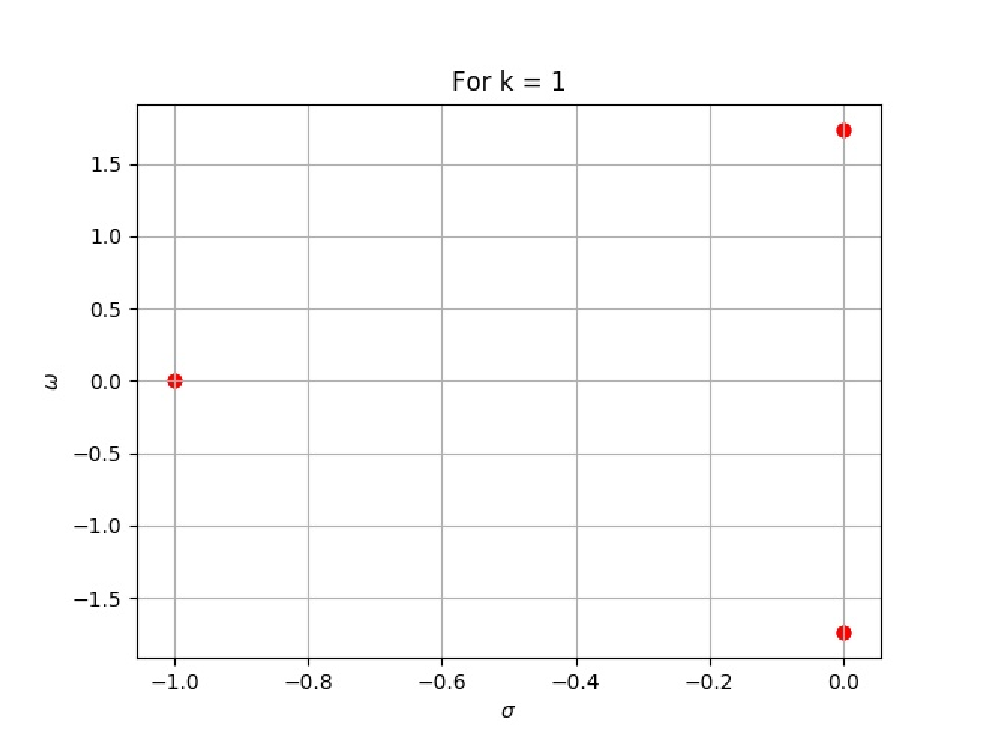
\includegraphics[scale = 0.5]{ee18btech11039_1.eps}
\end{center}
\label{fig:ee18btech11039}
\end{figure}

\begin{figure}[!ht]
\begin{center}
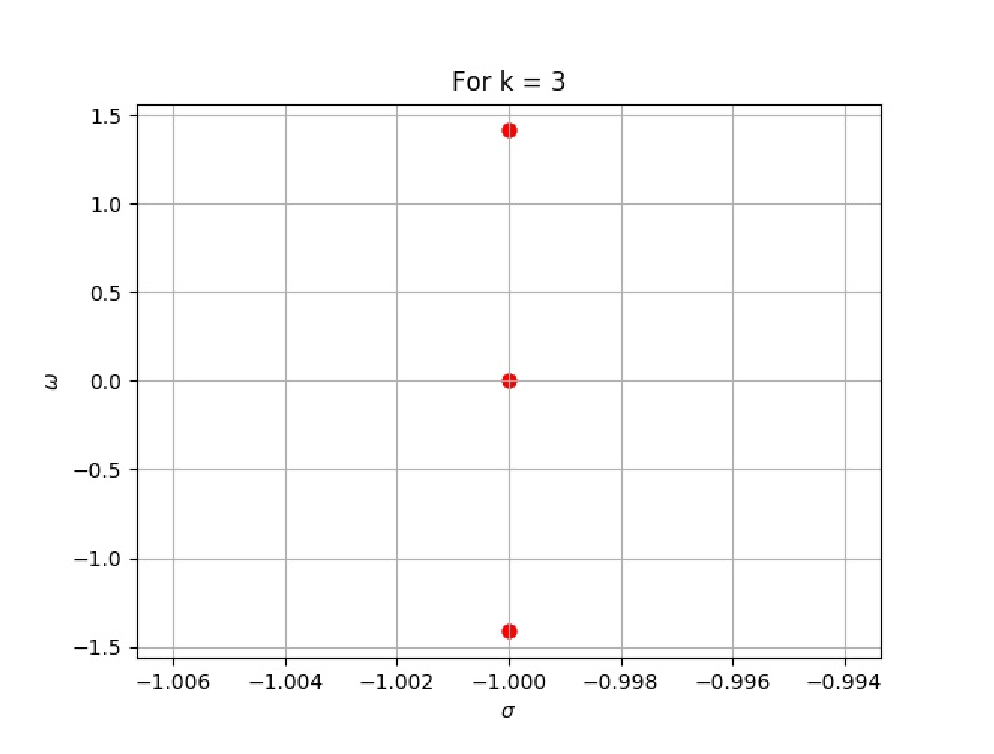
\includegraphics[scale = 0.5]{ee18btech11039_2.eps}
\end{center}
\label{fig:ee18btech11039}
\end{figure}

\begin{figure}[!ht]
\begin{center}
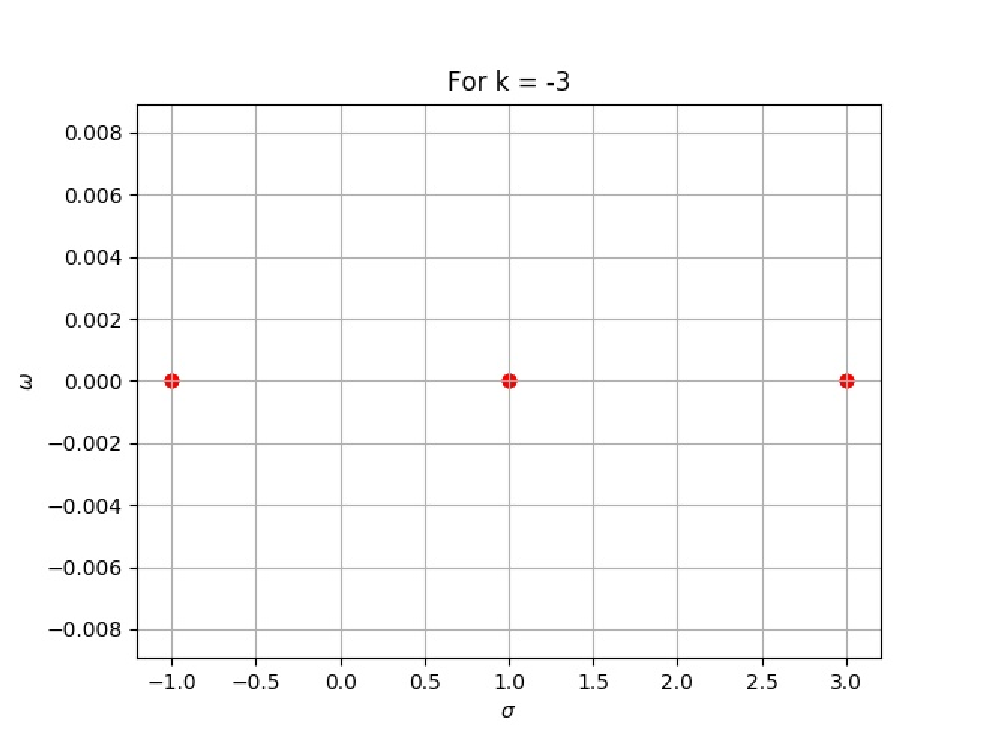
\includegraphics[scale = 0.5]{ee18btech11039_3.eps}
\end{center}
\label{fig:ee18btech11039}
\end{figure}


